\documentclass[12pt,a4paper]{report}
\usepackage[utf8x]{inputenc}
\usepackage[T1]{fontenc}
\usepackage{lmodern}
\usepackage{ucs}
\usepackage{amsmath}
\usepackage{amsfonts}
\usepackage{amssymb}
%\usepackage{fullpage}
\usepackage[french]{babel}
\usepackage{xcolor}
\usepackage[pdftex]{graphicx}
\usepackage{titlesec}
\usepackage{cite}
\usepackage{pdfpages}
\usepackage{url}
\usepackage{rotating}
\usepackage[top=2cm,bottom=2cm,left=2.5cm]{geometry}

%%%%%%%%%%%%%%%%%encadrementdes chapitres%%%%%%%%%%%%%%%%%%%%%%%
\titleformat{\chapter} % commande de sectionnement affectée
[frame] % une des formes prédéfinies
{\itshape} % format appliqué au titre dans son ensemble
{\filright\small\enspace Chapitre \thechapter\enspace} % format du « n° » du titre
{8pt} % distance (horiz. ou vert.) entre le n° et le texte du titre
{\Large\bfseries\filcenter} % format appliqué au texte du titre
%%%%%%%%%%%%%%%%%%%%%%%%%%%%%%%%%%%%%%%%%%%%%%%%%%%%%%%%%%%%%%%%
\newcommand{\HRule}{\rule{\linewidth}{0.5mm}}
\title{Rapport Projet de programmation}
%\author{Charlotte \textsc{Herice}\\ Typhaine \textsc{Paysan-Lafosse}\\ Thomas \textsc{Faux}\\ Joris \textsx{Sansen}}
% Commenté car provoque une erreur lors de la compilation
\begin{document}
%\maketitle
%\documentclass[10pt,a4paper]{report}
%\usepackage[utf8x]{inputenc}
%\usepackage{ucs}
%\usepackage{amsmath}
%\usepackage{amsfonts}
%\usepackage{amssymb}
%\usepackage{fullpage}
%\usepackage[french]{babel}
%\usepackage{xcolor}
%\usepackage{graphicx}
%\newcommand{\HRule}{\rule{\linewidth}{0.5mm}}
%\begin{document}

\begin{titlepage}

\begin{center}


% Upper part of the page

\includegraphics[width=0.15\textwidth]{logounibdx.png}\\[1cm]

\textsc{\LARGE Université de Bordeaux}\\[1.5cm]
\vspace*{0.5cm}
%\textsc{\Large Projet Tutoré}\\[0.5cm]
\textsc{\Large Initiation à la Recherche\\\ et/ou Développement}\\[0.5cm]
%\textsc{\Large Development Project}\\[0.5cm]

\vspace*{1cm}

% Title
\HRule \\[0.3cm]
{ \begin{Huge}
\bfseries Rapport du projet de programmation :
\end{Huge} \\ \begin{huge}
Développement d'un utilitaire de sélection de particules observées au microscope électronique
\end{huge}}\\[0.3cm]

\HRule \\[1.3cm]
% Author and supervisor
\begin{minipage}{0.4\textwidth}
\begin{center} \large
%\emph{Author:}\\
Thomas \textsc{Faux}\\
Charlotte \textsc{Héricé}\\
Typhaine \textsc{Paysan-Lafosse}\\
Joris \textsc{Sansen}\\
\end{center}
\end{minipage}
\begin{minipage}{0.4\textwidth}
\begin{flushright} \large
%\emph{Supervisor:} \\
M. Jean-Christophe\textsc{Taveau}
\end{flushright}
\end{minipage}

\vfill

\begin{center}
2011-2012
\end{center}
% Bottom of the page

\includegraphics[width=0.4\textwidth]{./banniere_cbmn.png}\\[1cm]
CBMN - UMR 5248 \\
B8 AVENUE DES FACULTÉS \\
F-33402 TALENCE CEDEX \\

%{\large \today}

\end{center}

\end{titlepage}
%\end{document}
\newcommand{\cme}{cryo-MET}
\newcommand{\java}{Java~{\tiny \texttrademark}}
\newcommand{\js}{JavaScript}
\newcommand{\imj}{ImageJ}

\begin{abstract}
Le contexte de ce projet est l'étude de morphologies de virus ou de patchs de virus observés au microscope électronique (ME) dans le cadre d'une prestation de services avec une société pharmaceutique. Le projet consiste en le développement d'un utilitaire qui sélectionne automatiquement les particules virales et les protéines membranaires dans les images de \cme. Cet utilitaire se présnete sous la forme d'un plugin \imj, écrit en  langage \java.
Il aborde notamment la création de l'interface utilisateur, les méthodes de piquages choisies et implémentées ainsi que l'organisation générale du programme. 
\end{abstract}

\tableofcontents
\chapter*{Introduction}

\addcontentsline{toc}{chapter}{Introduction}
Notre projet s'est déroulé au sein du laboratoire de Chimie et Biologie des Membranes et Nanoobjets de Bordeaux (CBMN~\cite{cbmn:url}).
Il s'agit d'un laboratoire de recherche public composé de douze équipes de recherche dont l'équipe \emph{Architecture des Complexes Membranaires et processus cellulaires} (ACMPC). %
Cette équipe, dirigée par O.\textsc{Lambert}, s'intéresse à l'architecture de complexes membranaires sur des structures de type protéine-liposome. C'est dans ce cadre d'étude que les chercheurs travaillent avec un \emph{cryo-microscope électronique à transmission} (\cme) afin d'obtenir des micrographes des structures protéiques puis de les analyser. Par ailleurs, cette équipe diversifie ses activités en faisant de l'imagerie avec des virus fournis par une entreprise pharmaceutique.

\noindent
Cependant la nouvelle génération de \cme ~permet une collecte de données à haut débit, avantage non négligeable mais qui pose le problème du temps de traitement des données collectées. %

\paragraph*{}
Dans le cadre de leurs recherches et pour la partie qui nous intéresse, l'analyse concerne le traitement des images récupérées du \cme\ et plus particulièrement au \emph{picking}, c'est-à-dire au piquage des particules présentes sur les micrographes obtenus. %
Notre objectif était l'implémentation d'une plateforme contenant plusieurs méthodes de piquage automatisées.
Celle-ci est implémentée en \java ~\footnote{\java\ est un langage orienté-objet développé par Oracle~\cite{java:url}} sous la forme d'un plugin \imj~\cite{imagej:url}: elle propose à l'utilisateur des algorithmes de picking pré-installés ou d'en ajouter de nouveaux.

\paragraph*{}
Dans la suite de ce rapport, nous développerons plusieurs points. Tout d'abord une partie Analyse dans laquelle nous remettrons notre projet dans son contexte et analyserons les besoins liés à celui-ci. Ensuite, une partie Conception dans laquelle nous expliquerons l'organisation de notre code. Enfin, la partie Réalisation contiendra les solutions apportées au sujet.

\chapter{Analyse}

\section{Contexte}

\subsection{Présentation du CBMN}

Le laboratoire, créé en janvier 2007, est à l'interface entre le Biologie, la Chimie et la Physique. Il a pour tutelle les départements de Chimie et des Sciences de la Vie du Centre National de la Recherche Scientifique (CNRS) et les Unités de Formation et de Recherche (UFR) de Chimie et de Biologie de l'Université Bordeaux I, II et l'ENITAB. \\
La mission du CBMN est d'apporter une connaissance fondamentale de phénomènes biologiques complexes en les analysant à plusieurs échelles, allant de la molécule à la cellule et à l'organisme. \\
L'équipe ACMPC s'appuie sur deux méthodes d'imagerie : la cryotomographie  électronique et la microscopie à fluorescence. Comme nous l'avons expliqué précédemment, nous allons travailler sur des images issues de cryomicroscopie.  

\subsection{Objectifs}

\noindent
Notre objectif était de créer et d'implémenter une plateforme mettant à disposition plusieurs méthodes de piquage automatisées des particules sur les micrographes. Les échantillons qui nous ont servi de tests étaient de deux types :%
\begin{itemize}
\item des micrographes d'échantillons de virus, de forme ronde, qu'il fallait sélectionner afin de pouvoir déterminer leurs nombre et tailles,
\item des micrographes de protéines membranaires, de forme pyramidale, qu'il fallait aussi sélectionner.\\
\end{itemize}
\noindent
Il était imposé que cette interface soit implémentée sous la forme d'un plugin ImageJ. Elle propose à l'utilisateur de se servir des algorithmes de picking pré-installés. \\%

\noindent
Le logiciel ImageJ a été choisi car c'est un logiciel de traitement et d'analyse d'images développé en \java~\footnote{\java\ est un langage orienté-objet développé par Oracle~\cite{java:url}} par le Nation Institute of Health (NIH).%

\noindent
Ce logiciel est "open-source"~\footnote{son code source est en accès libre et est modifiable(licence GNU-GPL)}, multi-plateforme et bien connu de la communauté scientifique car initialement conçu pour des applications biomédicales. Il s'est peu à peu démocratisé dans d'autres domaines pour sa facilité d'utilisation et les possibilités de développement qu'il offre.%

\noindent
En effet, il est possible de développer soi-même et assez facilement des plugins, que ce soit en \java\ ou en \js ~\footnote{\js est un langage de programmation de script orienté objet à prototype~\cite{javascript:url}}.

\section{\'Etat de l'existant}

\subsection{Détection à l'aide de références}

Cette technique est utilisée pour trouver des particules dans une image en la comparant à un modèle. Celui-ci peut \^etre obtenu soit à partir d'une structure tridimensionnelle connue, soit par sélection d'une particule servant d'exemple dans le micrographe. L'algorithme détermine la meilleure correspondance entre la cible et le modèle pour pouvoir le localiser dans l'image.%

\subsection{Piquage de particules sans références}

\subsubsection{Détection des bords et transformée de Hough}

%$\textcolor{red}{(ref:Automatic Particle Detection Through Efficient Hough Transforms
%by Yuanxin Zhu, Bridget Carragher, Fabrice Mouche, and Clinton S.Potter
%IEEE TRANSACTIONS ON MEDICAL IMAGING,VOL.22,N0.9,September 2003)}$\\


%$\textcolor{red}{(ref:http://en.wikipedia.org/wiki/Hough_transform)}$\\
\paragraph*{}
Les difficultées majeures rencontrées dans les techniques basées sur la détection des contours sont dues à la compléxité de détecter les bords des particules lorsqu'il y a un bruit de fond important sur les images issues de la Microscopie à Transmission Electronique.%

\noindent
Cette technique est basée sur la détection des arêtes ainsi que sur l'application de la transformée de Hough~\cite{PdetectEHT:article}. Cette méthode permet de détecter la présence de formes comme des lignes, des cercles ou encore des ellipses.%

\noindent
Dans la transformée de Hough\cite{HT:url} appliquée à la détection de lignes, pour chaque pixel allumé de l'image on trace toutes les lignes possibles, on obtient alors une sinusoïde unique appelée espace de Hough. Si les courbes associées à deux points se coupent, l'endroit où elles se coupent dans l'espace de Hough correspond aux paramètres d'une droite qui relie ces deux points (ordonnée à l'origine et pente).%

\paragraph*{}
La détection de formes s’apparentant à des cercles ou des axes circulaires se fait en détectant le centre de celles-ci.
Pour chaque pixel allumé, la fonction trace un cercle de rayon donné. Si la forme a le même rayon que le cercle tracé, tous les cercles se recoupent au centre de la forme, on constate ainsi une amplification de la valeur du pixel central.

\paragraph*{}
D'autre part, pour détecter des particules de formes irrégulières, l'approche décrite précédemment peut également \^etre utilisée mais la transformée de Hough devra alors \^etre remplacée par la transformée de Hough Généralisée~\cite{GHT:url}.
Cette nouvelle méthode repose sur la modification de la transformée de Hough en utilisant le principe de l'identification à partir d'un modèle de référence.
%$\textcolor{red}{(ref:http://en.wikipedia.org/wiki/Generalised_Hough_transform)}$\\

\subsubsection{DoGLFC et classement par affinité}

%$\textcolor{red}{(ref: Reference-free particle selection enhanced with semi-supervised machine learning for cryo-electron microscopy
%by Robert Langlois, Jesper Pallesen, Joachim Frank
%Journal of Structural Biology 175, (2011)353-361)}$
\paragraph*{}
Cette technique est basée sur l'utilisation de l'algorithme DoGLFC\footnote{Difference Of Gaussian Local Fast Correlation} complété par l'algorithme de classement par affinité~\cite{DoGAff:article}.

\paragraph*{}
Le DoGLFC est basé sur l'algorithme DoG Picker du Scripps Institute\cite{Scripps:url}, une méthode rapide qui permet la segmentation de particules. Après l'application de l'algorithme de Différence de Gauss (DoG), on obtient une cartographie de points similaire à celle de la méthode utilisant un modèle de référence.%\blue {\Large ?!} \black %

\noindent
Cet algorithme requiert un paramètre ajustable unique ou un jeu de paramètres basé sur le rayon de la particule ou un ordre de grandeur du rayon. L'exécution de cet algorithme renvoie une liste de trois paramètres décrivant la localisation de la particule (les coordonnées \emph{x} et \emph{y}) et la taille du pic.%

\noindent
L'algorithme DoGLFC sélectionne les particules (ou objets) potentielles de taille déterminée, ceci a un pouvoir discriminatif moindre par rapport à une technique basée sur un modèle de référence.

\paragraph*{}
Pour améliorer le rendement lors du piquage des particules, un nouvel algorithme semi-supervisé, le classement par affinité, peut \^etre appliqué.

\noindent
L’algorithme a besoin de trois paramètres d'entrée: un jeu d'images, la taille minimale de l'image après réduction et deux références indiquant quelle fen\^etre doit \^etre utilisée comme référence positive ou négative.

\noindent
Lorsque l'algorithme a fini de se dérouler, on obtient une classement pour chaque fen\^etre où le maximum correspond à la particule ciblée.

\paragraph*{}
L'utilisation de DoGLFC complété par le classement par affinité permet d'extraire
rapidement les particules de l'image et d'éliminer avec précision les particules correspondant à de la contamination ou du bruit de fond.

\subsection{Perceptron}

\paragraph*{}
Un perceptron est une sorte de réseau neuronal artificiel. Dans son état le plus simple, il représente un système de classification binaire/linéaire.%

\noindent
Ce programme a la particularité d'être capable d'apprendre des concepts, ce qui signifie qu'il peut apprendre afin de répondre par vrai ou faux à des données qui lui sont soumises, gr\^ace à la présentation répétée de plusieurs exemples d'étude.
Il a déjà été testé sur des images binaires pour la détection de formes ou de contours mais pas sur des images en niveaux de gris ou sur des problèmes de reconnaissance de modèles visant à sélectionner des particules. Le réseau neuronal n'a pas non plus été exploité comme un outils de sélection automatique de particules mais plusieurs recherches ont conclu qu'il pourrait \^etre utilisé pour l'élimination de faux-positifs.~\cite{Perceptron:article}.%

\section{Analyse des besoins}

\noindent
Ils sont de deux types: fonctionnels et non fonctionnels, et diffèrent entre l'interface utilisateur et les algorithmes de piquage.

\subsection{Besoins fonctionnels}

\subsubsection{Interface}

\noindent
Au lancement, les images sont préalablement chargées sur \imj , l'utilisateur a le choix entre plusieurs algorithmes de picking. %L'interface propose un mode de prévisualisation afin de vérifier le piquage sur une image avant de l'appliquer au stack entier.
Nous avons essayé de faire en sorte que l'affichage soit clair et succinct, constitué d'un menu déroulant, d'une liste de boutons et d'une interface propre à chaque algorithme.\\
Enfin, il est également possible d'implanter simplement de nouveaux algorithmes dans l'interface. % Simplement, ou pas ^^

\subsubsection{Les algorithmes}

Ils réalisent un piquage automatique des particules depuis les micrographes issus de \cme. Le format de sortie est un tableau de résultats contenant un jeu de coordonnées \emph{x, y} associé à la position de l'image dans le stack, ainsi qu'un mini-stack contenant les particules sélectionnées par l'algorithme si l'utilisateur le désire.

\subsection{Besoins non fonctionnels}

\subsubsection{Interface}

\noindent
L'implémentation de la plateforme a été réalisée en \java, nous utilisons les API\footnote{Application Programming Interface} graphiques de la bibliothèque \emph{Swing}. 
Il s'agit d'une interface graphique (GUI)\footnote{Graphic User Interface} faisant partie du paquage Java Foundation Classes (JFC), inclus dans J2SE. Swing constitue une des principales évolutions apportées par Java2 par rapport aux versions antérieures. Elle offre la possibilité de créer des interfaces graphiques identiques quelque soit de système d'exploitation sous-jacent, au prix de performances moindres qu'en utilisant Abstract Window Toolkit (AWT) l'autre bibliothèque principale pour \java. \\
De plus, nous avons essayé de faire en sorte que le programme soit le plus simple d'utilisation possible afin de le rendre accessible à tous. C'est pourquoi nous avons tenté de faire un code clair, explicite et commenté afin de permettre aisément l'implémentation de nouveaux algorithmes.

\subsubsection{Les algorithmes}

\noindent
Les algorithmes ont été testés avec l'outil macro d' \imj ~puis implémentés en \java, nous avons fait en sorte que le temps de déroulement de l'algorihtme soit assez rapide afin de pouvoir gérer de grands jeux de données et qu'aucune image de traitement intermédiaire n'apparaisse à l'utilisateur (à moins qu'il ne le souhaite).\\

Dans l'optique de démocratiser l'utilisation de notre interface et afin de permettre l'extension de ce plugin avec d'autres algorithmes, le projet a été placé sous une licence GPL\footnote{General Public License~\cite{GPL:url}}.

\noindent
%Le projet devra être terminé vers mi-mai. %prière de nous mettre une bonne note !

\section{Scénario d'utilisation du plugin}

Nous prendrons l'exemple d'une image issue de \cme ~sur laquelle se trouvent des protéines membranaires que nous voulons sélectionner (Figure \ref{prot}) ainsi que d'une image utilisée comme référence sur \imj ~, les \emph{blobs} (Figure \ref{blobs1}).

\begin{figure}[!ht]
\begin{center}
 \begin{minipage}{.450\linewidth}
  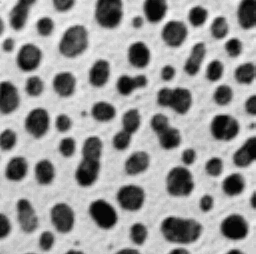
\includegraphics[width=0.92\textwidth]{blobs.png}  
  \caption{Image Blobs de réference}
  \label{blobs1}
 \end{minipage} \hfill
\begin{minipage}{.450\linewidth}
  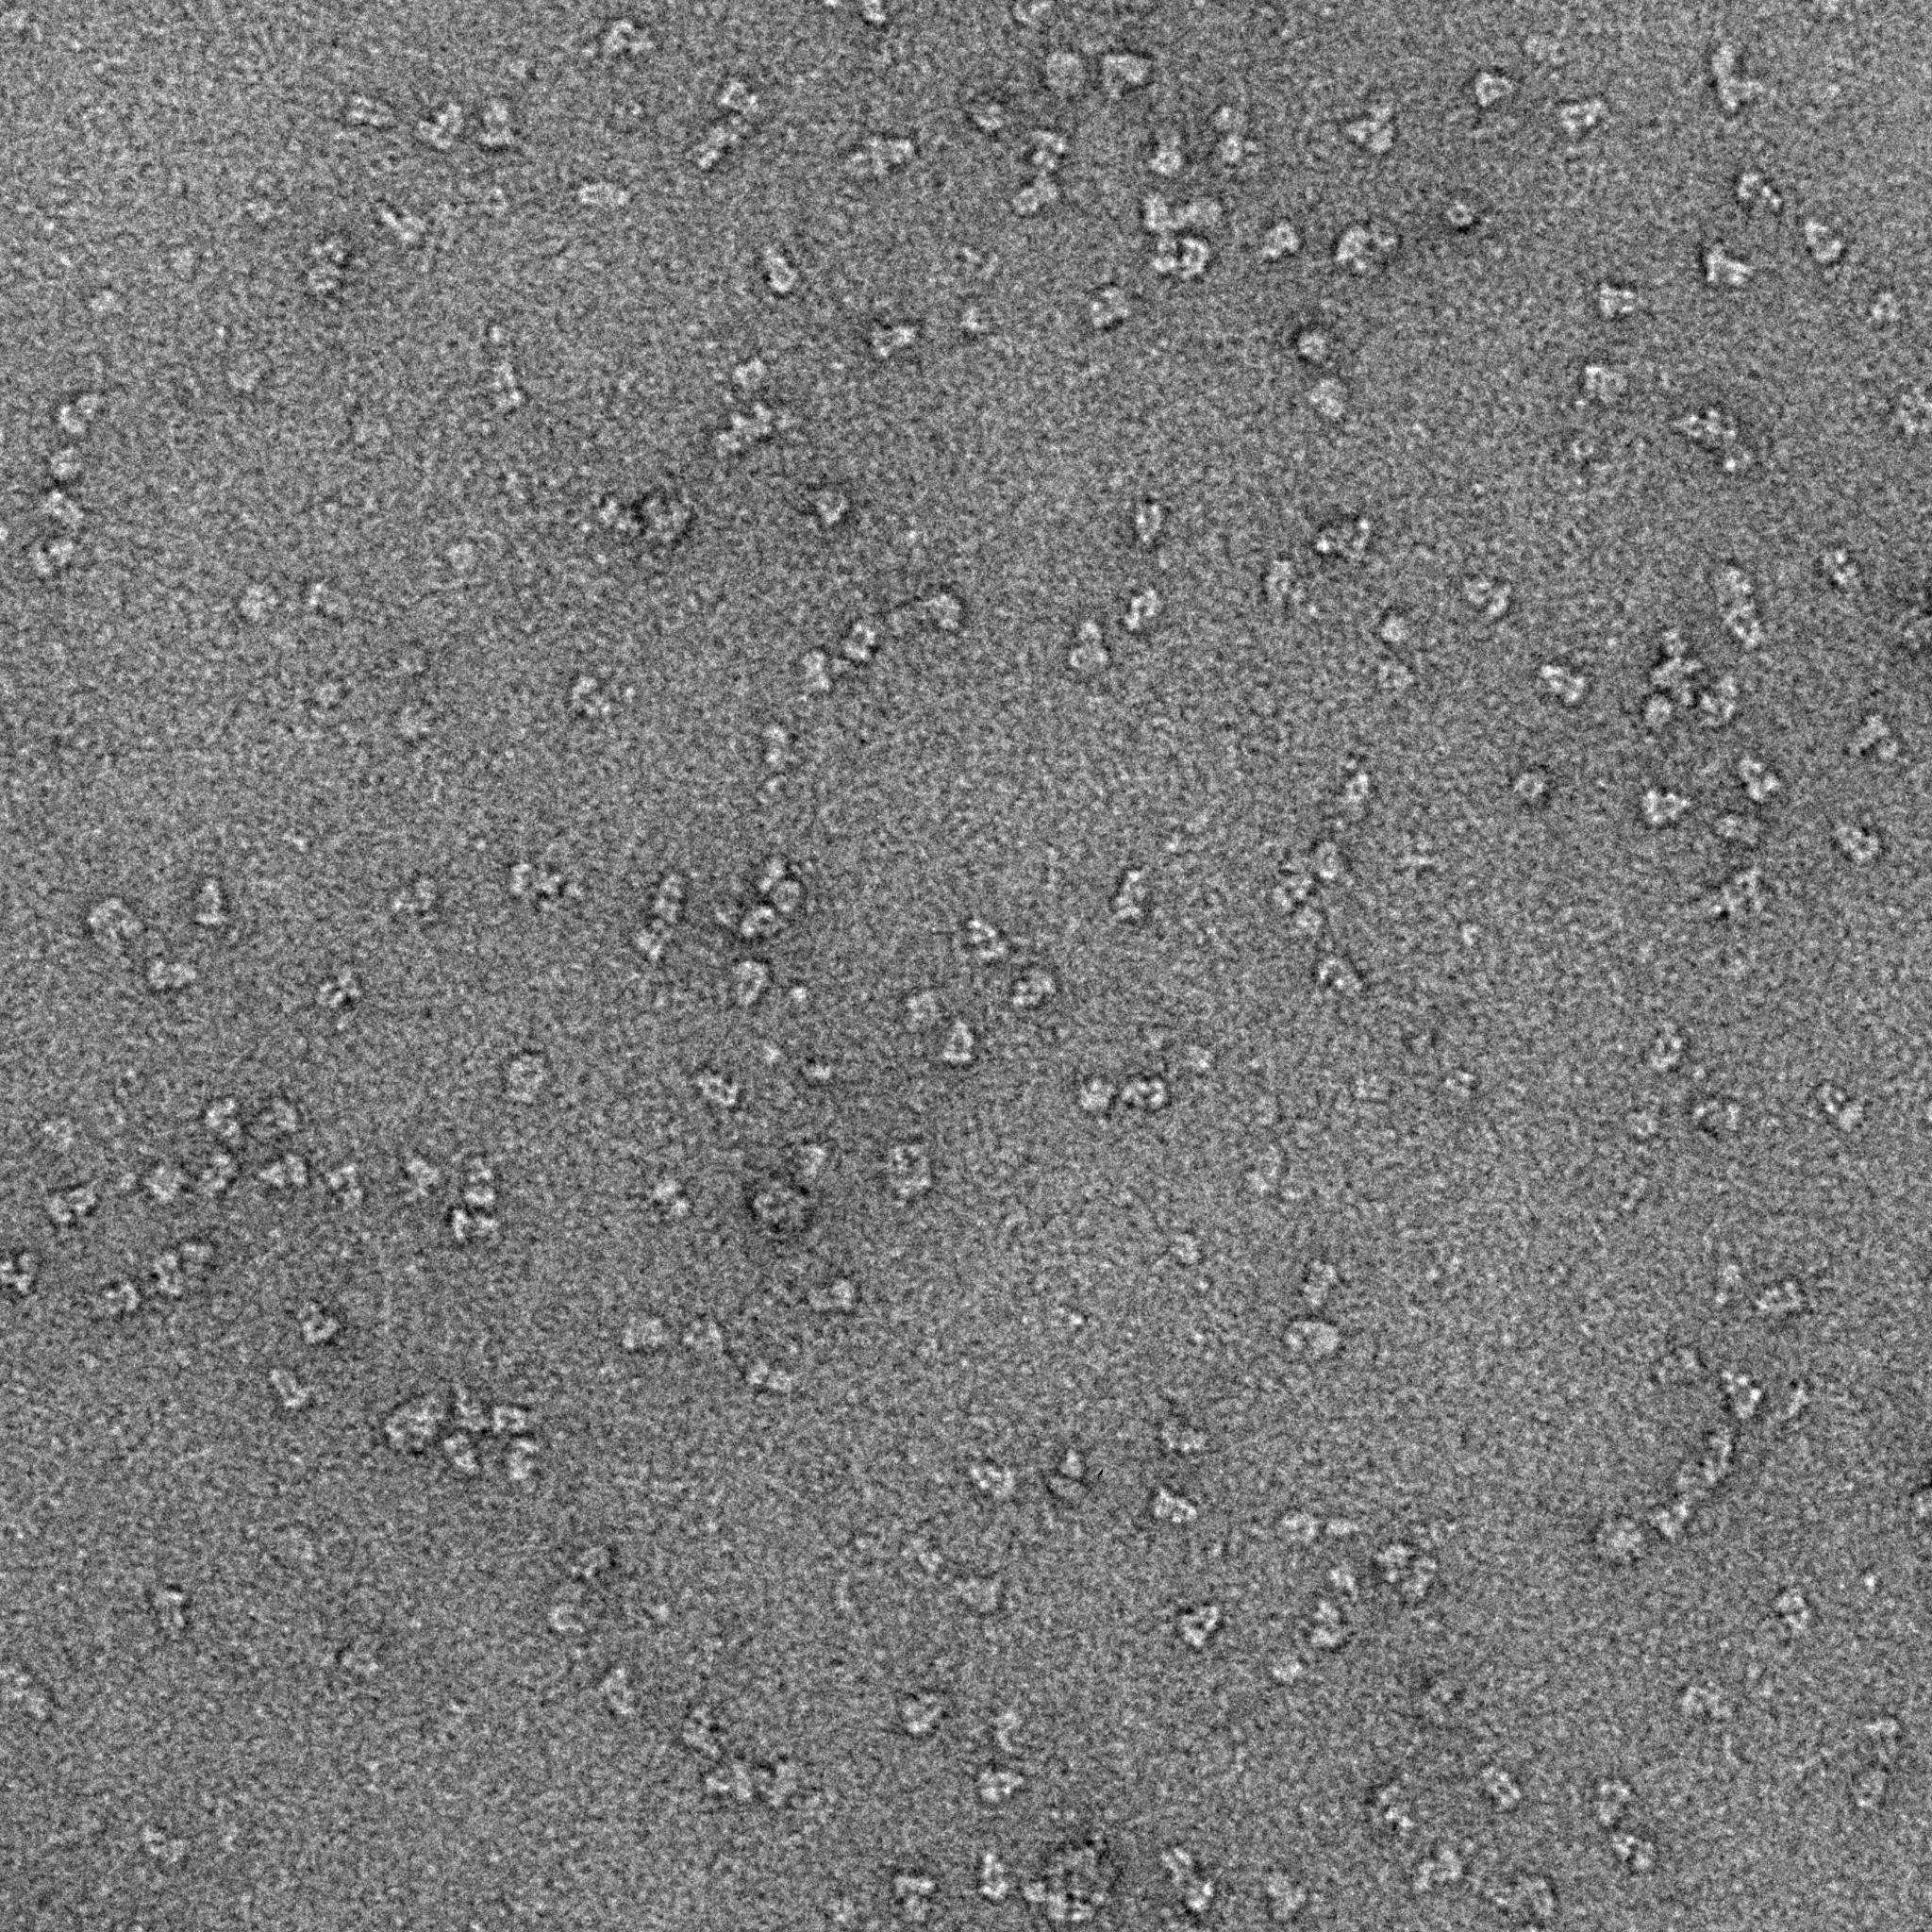
\includegraphics[width=0.98\textwidth]{proteines.jpg}   
  \caption{Image de protéines membranaires observées au \me}
  \label{prot}
 \end{minipage} \hfill
%\caption{Exemple d'images formant le stack de particules (blobs et protéines)}
\end{center}
\end{figure}

%\begin{figure}[h] 
%\begin{center}
%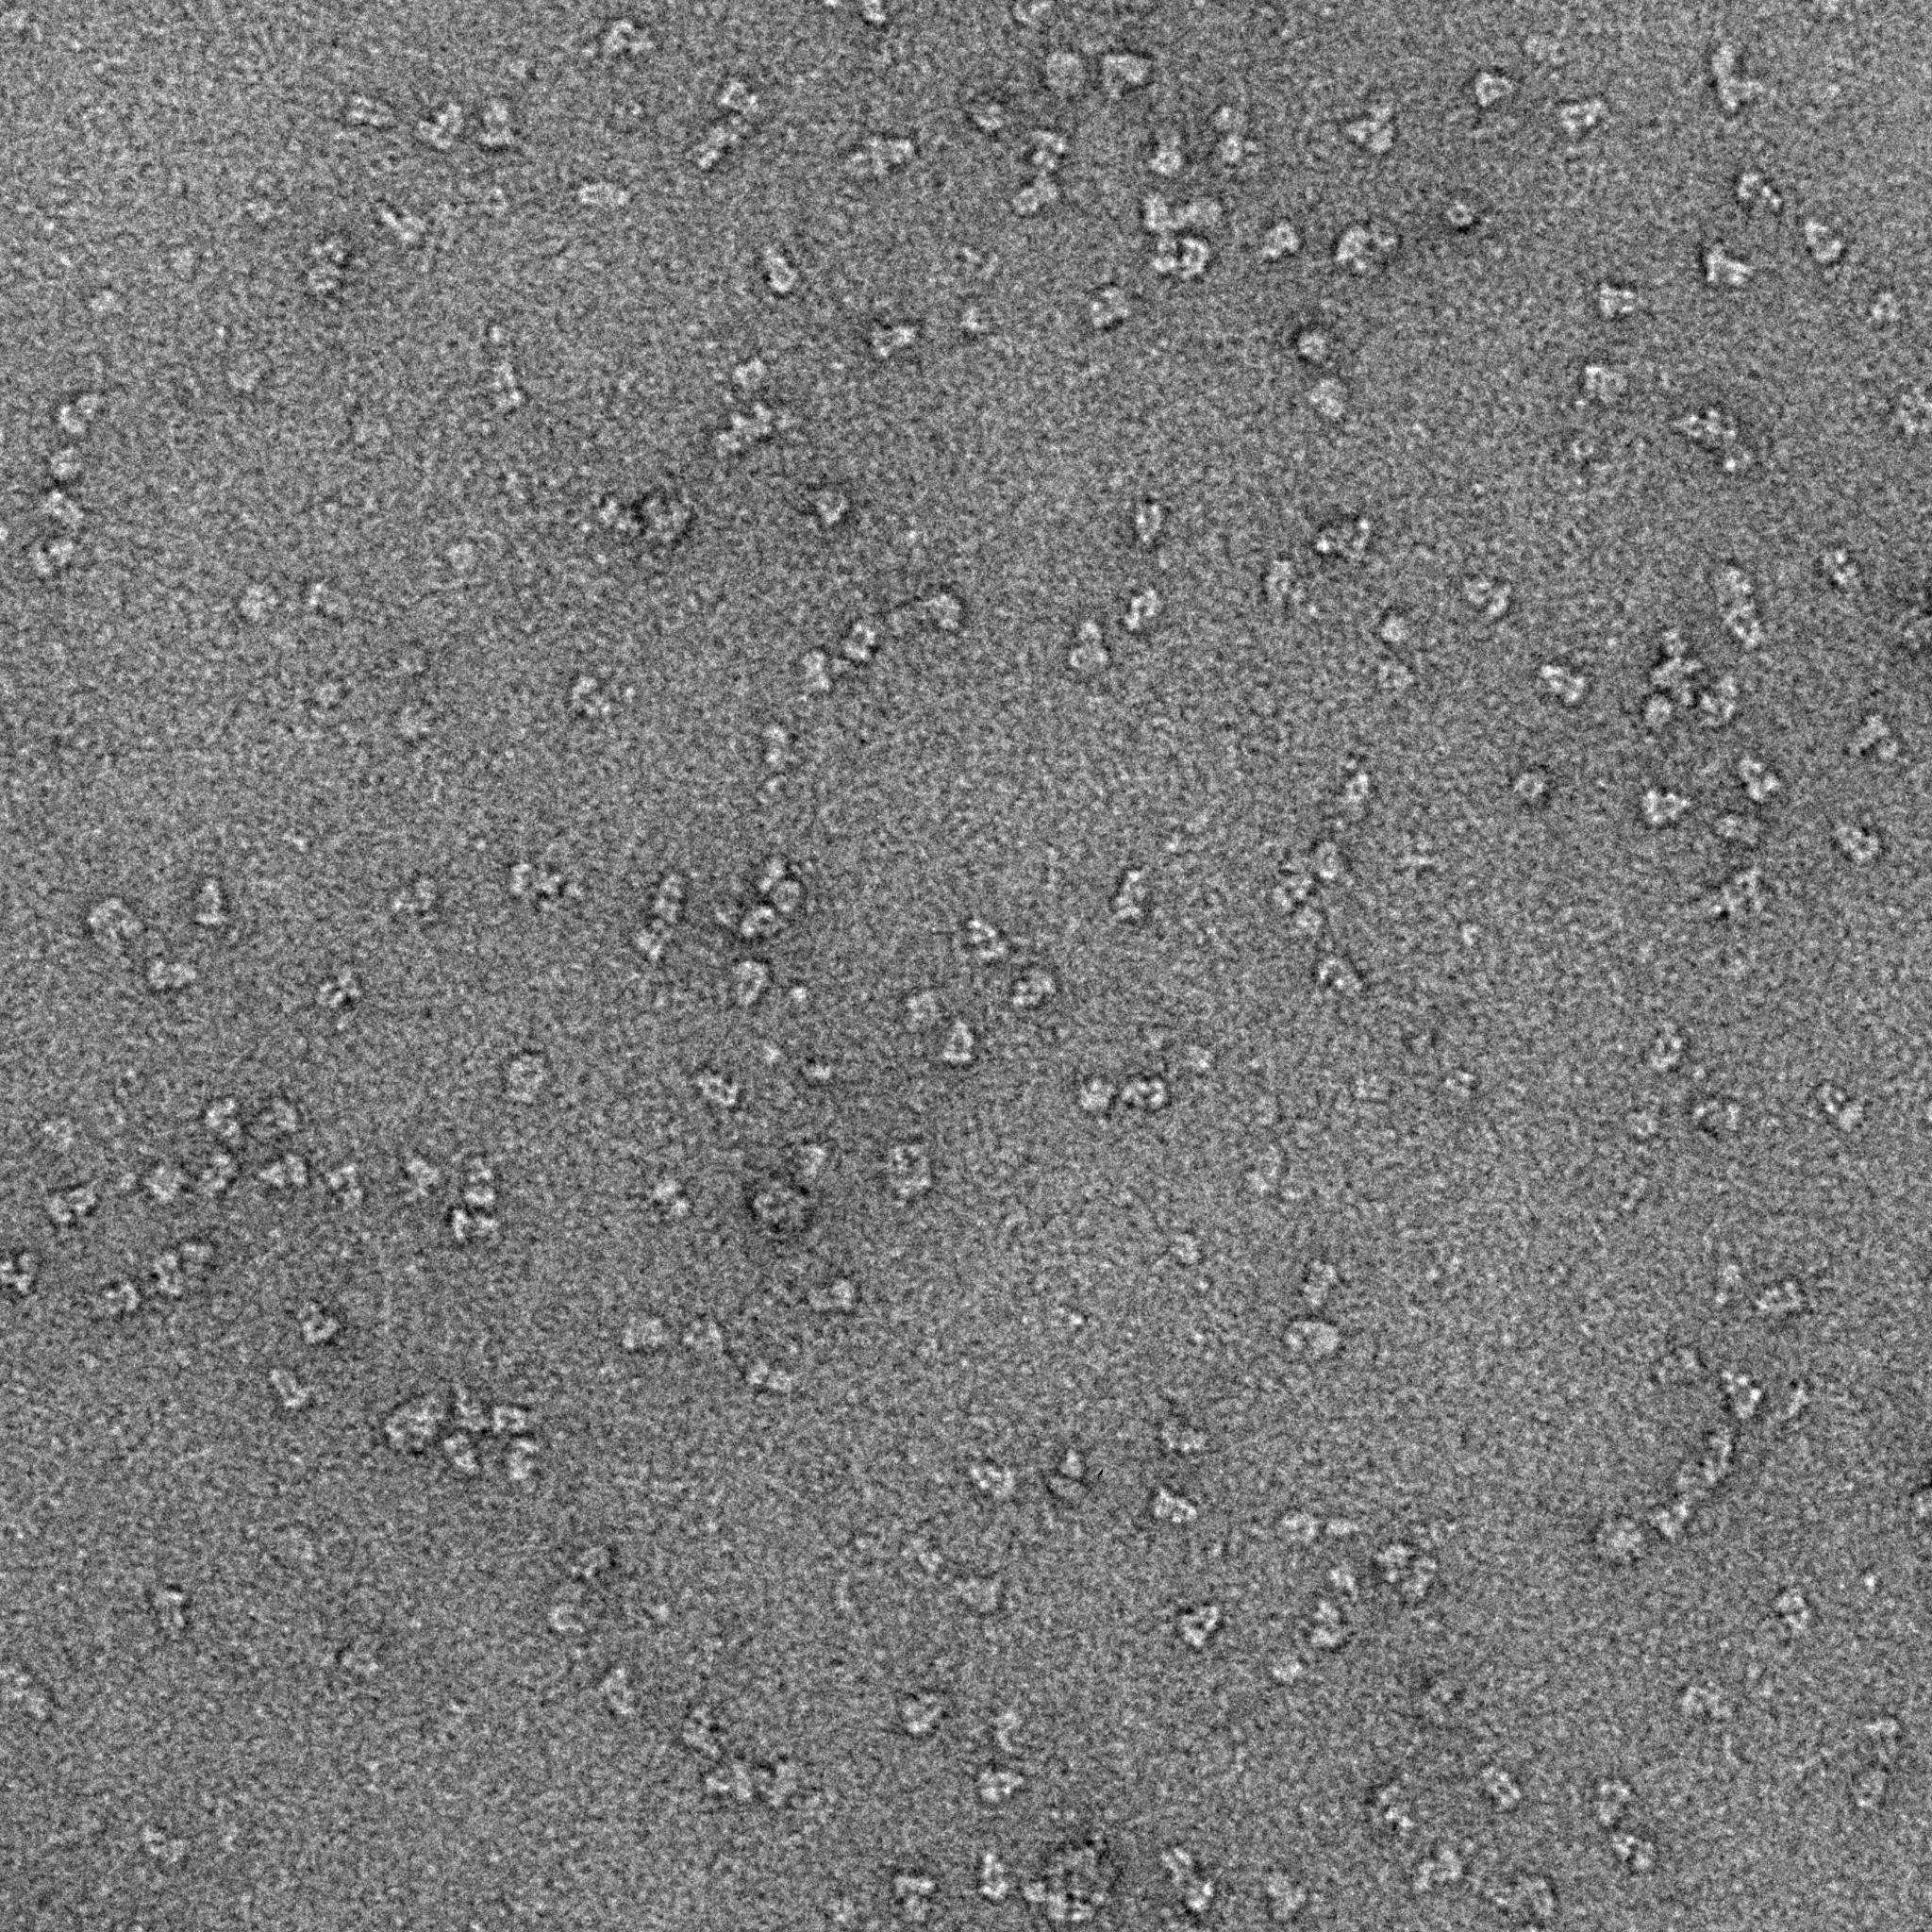
\includegraphics[width=0.5\textwidth]{proteines.jpg}
%\caption{Image de protéines membranaires observées au \me}
%\label{prot}
%\end{center}
%\end{figure}

Nous avons tenté de nous mettre à la place d'un chercheur pour avoir une vision biologique de l'utilisation de notre plugin. Tout au long de ce rapport, vous pourrez donc suivre toutes les procédures qui nous ont permis de réaliser la sélection. 


\chapter{Conception}

\section{Généralités de conception}
\subsection{L'interface graphique}
Comme précisé précédemment, notre programme se présente sous la forme d'un plugin \imj . L'interface graphique à été réalisée grâce à la bibliothèque  \java ~Swing, %Il a été réalisé grâce à la bibliothèque Swing de \java ~pour l'interface graphique.
La fenêtre servant d'interface est composée de differentes boites (panneaux). Ces boites contiennent différents outils (boutons, listes, zones de saisie et zones de texte) permettant l'interaction entre l'utilisateur et le programme. Les boîtes peuvent s'imbriquer les unes dans les autres afin d'obtenir des structures plus complexes et un meilleur rendu visuel. \\
%Nous avons donc créé une série d'outils graphiques (boutons, listes, zone de saisie et zone de texte) pour l'interaction avec l'utilisateur. Dans une fenêtre, ces outils sont disposés en lignes ou en colonnes dans des boîtes (panels). Les boîtes peuvent s'imbriquer les unes dans les autres afin d'obtenir des structures plus complexes et un meilleur rendu visuel. \\
L'interface du plugin est simple, elle prend la forme d'une fenêtre composée d'un menu déroulant, dans lequel se trouvent les différents algorithmes, et de quatre boutons. \\

\subsubsection{Les panneaux}

Notre interface est composée d'une arborescence de panneaux organisée comme suit : \\
Un panneau principal, permettant d'organiser la fenetre du plugin, composé des trois panneaux subsidiaires suivant :
%Notre interface est composée de quatre panneaux différents (voir Figure \ref{panneaux}) :
\begin{description}
\item [Le premier panneau] contient une liste déroulante permettant le choix de l'algorithme. 
%\item Le panneau en haut de la fenêtre contient une liste déroulante pour le choix de l'algorithme. 
\item [le panneau du milieu] est vide au lancement du plugin et s'actualise en fonction de l'algorithme de piquage choisi.\\
Il affiche une aide rapide sur les condition d'utilisation de l'algorithme de piquage, les zones de saisies utilisateur propre à cet algorithme, les choix génériques : mode de deboggage, mode de découpe des selections et taille de la selection, gestion du bruit de fond. Tout cela s'organise à l'aide de sous-panneaux.
%\item Le panel du milieu est vide au lancement du plugin et son contenu s'actualise en fonction de l'algorithme de piquage choisi. Il contient 4 sous-panneaux :
%\begin{itemize}
%\item Le premier sous-panneau contient une zone de texte visant à guider l'utilisateur sur la manière de lancer la procédure de piquage choisie. 
%\item Le deuxième sous-panneau se situe au milieu et change en fonction de l'algorithme choisi. Il conporte un nom différent suivant l'algorithme choisi : il va se nommer \textbf{iterationPanel} pour Dilate Difference, \textbf{sigmaPanel} pour Difference of Gaussian et \textbf{radiusPanel} pour Image Correlation. Ces sous-panels contiennent deux ou trois TextFields (zones de texte à une seule ligne) pour que l'utilisateur puisse entrer les valeurs des paramètres nécessaires au bon fonctionnement des algorithmes. 
%\item Le troisième sous-panel (\textbf{widthNoisePanel}) quand à lui contient deux TextFields pour les paramètres \textbf{Square width} et \textbf{Noise Tolerance} sur lesquels nous reviendrons par la suite. 
%\item Le dernier sous-panel (\textbf{debugCropPanel}) contient deux checkboxs pour les modes de debug et crop (voir plus loin dans le rapport). 
%\end{itemize}
\item [le dernier panneau] contient les boutons d'actions : prévisualisation, éxécution, affichage des résultats, informations/aide.
%\item Le panel en bas de la fenêtre (\textbf{panel3}) contient quatre boutons qui permettent à l'utilisateur de faire fonctionner le plugin. 
%\item Le panel principal (\textbf{mainPanel}) contient tous les panels cités précédemment. Sa taille détermine celle de la fenêtre du plugin. 
\end{description}
Le panneau principal permet notamment d'imposer la taille de l'interface.\\
La figure suivante (\ref{panneaux}) donne un aperçu plus visuel de l'organisation de ces différents panneaux.
\begin{figure}[!h] 
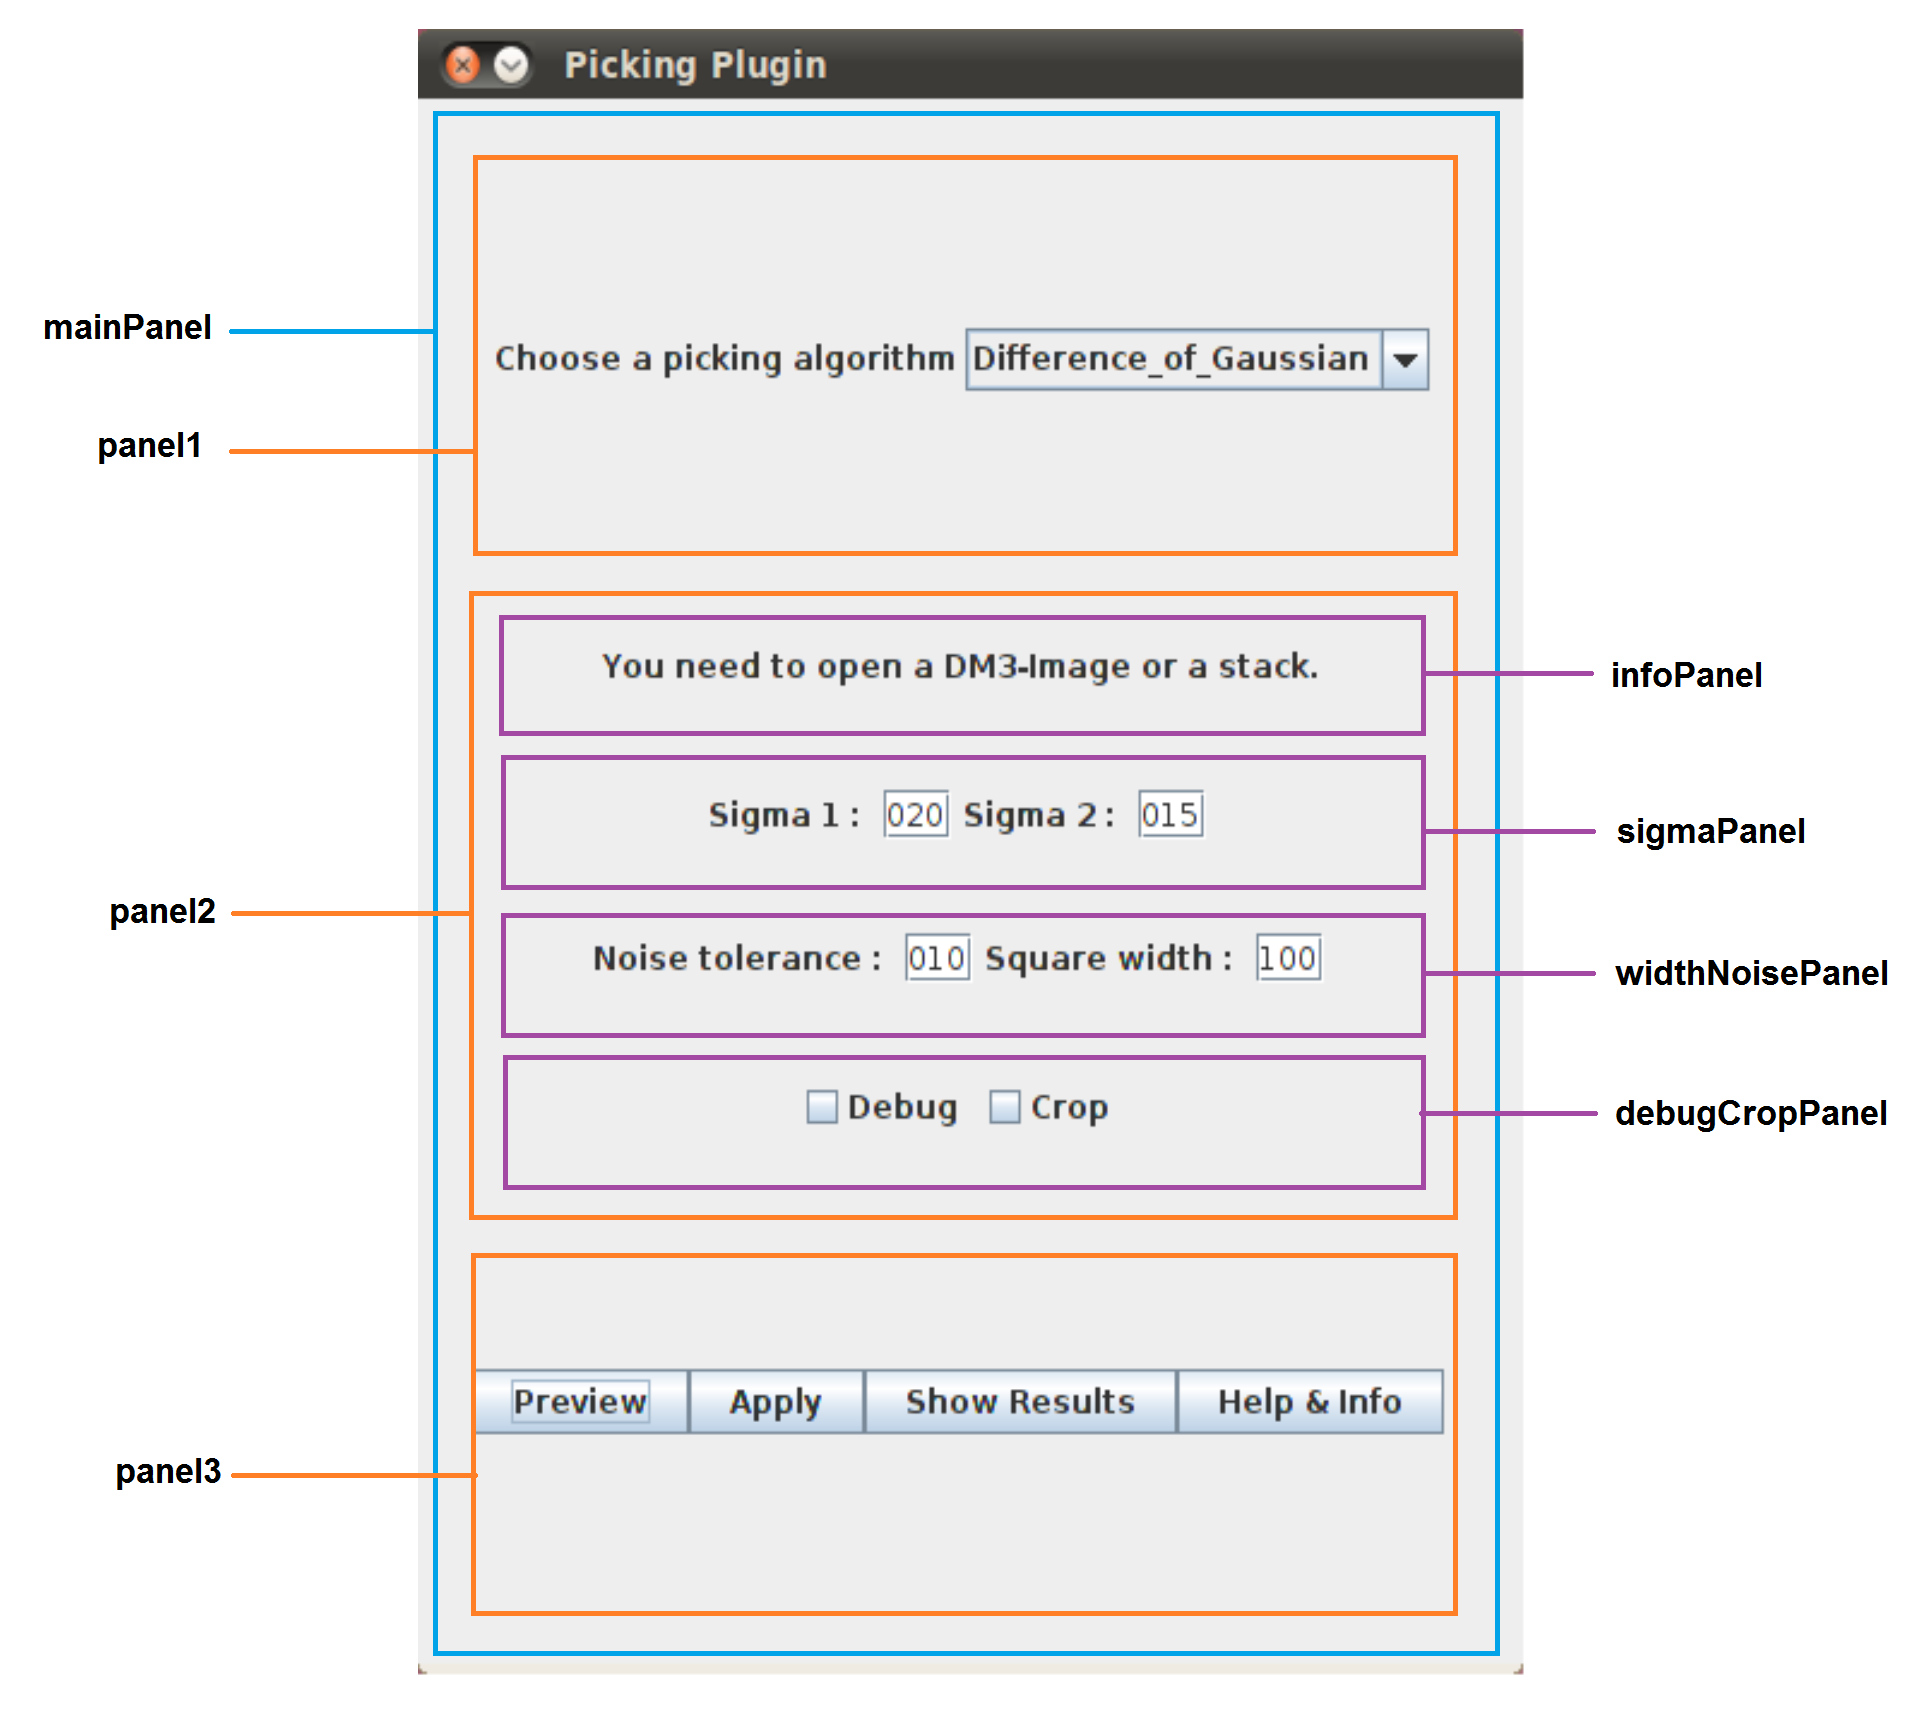
\includegraphics[width=1\textwidth]{plugin3-1.png}
\caption{Organisation des panels pour l'algorithme Difference of Gaussian}
\label{panneaux}
\end{figure}
\pagebreak
\subsubsection{Les boutons}

Les boutons doivent répondre aux clics de la souris et lancer l'action correspondante en fonction de l'algorithme de piquage choisi par l'utilisateur :

\begin{description}
\item [Le bouton de prévisualisation] permet de tester le piquage obtenu par l'algorithme sélectionné sur l'image courante.
\item [Le bouton d'éxécution] permet d'appliquer l'algorithme sur l'image ou le stack séléctionné, lorsque l'utilisateur est s\^ur des paramètres qu'il souhaite appliquer.
\item [Le bouton d'information/aide] est une aide d'utilisation du plugin ainsi que des conditions de fonctionnement des algorithmes.
\item [Le bouton d'affichage des résultats] permet d'afficher et de sauvegarder le tableau des coordonnées des particules sélectionnées.% avec l'aide d'\imj.  
\end{description}
Pour que le plugin puisse fonctionner, l'utilisateur devra au préalable avoir ouvert une image ou un stack d'images à l'aide d'\imj.
\pagebreak
\subsection{les algorithmes}
L'utilisateur sélectionne un algorithme dans le menu déroulant et détermine certains paramètres :\\
%Lorsque l'utilisateur sélectionne un algorithme dans le menu déroulant, il doit choisir plusieurs paramètres.
Certains sont communs à tous tel que :
\begin{itemize}
\item la gestion du bruit de fond,
\item la taille des images des particules sélectionnées lorsqu'on demande le stack d'images,
\item activation du deboggage (s'il est implémenté dans l'algorithme),
\item activation du découpage des particules à partir du piquage obtenu.
\end{itemize}
D'autres sont propres aux algorithmes.
\subsubsection{Correlation d'image}
Le principe de cette méthode est de corréler une image de cercle d'une taille définie avec notre image de base convertie en image binaire. Pour chaque pixel noir on trace le cercle avec ce pixel pour centre.
Si le cercle est de la m\^eme taille que la particule, les cercles se croiseront tous au centre de cette particule formant un point blanc central. On obtient donc une image résultante de corrélation présentant des maxima blancs au centre de chaque particules dont la taille est identique à celle du cercle.\\
Cet algorithme trouve donc les valeurs élevées de pixel correspondant à la meilleure superposition locale entre l'image de référence (le cercle) et l'image de base.\\

%Le principe de cette méthode est de comparer une image contenant un cercle avec l'image sur laquelle on veut sélectionner les particules. On obtient alors une nouvelle image sur laquelle on peut voir des cercles correspondant aux particules de l'image de base qui ont à peu près le même diamètre que le cercle dessiné précédemment. Ici, on fait varier la taille du cercle afin de sélectionner des particules de différentes tailles.\\
\noindent
Pour cette méthode de piquage, l'utilisateur doit donc entrer le rayon minimal et maximal des particules à sélectionner, ainsi que la valeur de l'incrémentation.\\ Pour un résultat optimal, avant de lancer la sélection des particules avec cet algorithme, l'utilisateur devra traiter l'image pour éliminer un maximum de bruit de fond (utilisation de filtres).

\subsubsection{Différence de Gaussienne}
La différence de Gauss est une technique qui consiste en la soustraction d'une image à laquelle à été appliqué un filtre gaussien à une deuxième image moins filtrée avec un écart-type plus petit. Les bords des particules sont donc dégradés nous permettant de récupèrer les maxima de l'image résultante, c'est-à-dire les centres des particules.\\
%La différence de Gauss est une technique qui consiste en la soustraction d'une version floutée %de l'image d'origine à une autre version moins floutée de cette même image.\\
\noindent
On demande à l'utilisateur d'entrer les valeurs d'écart-type qui seront utilisés pour appliquer les filtres gaussiens.

\subsubsection{Différence de dilatation}

Cette méthode repose sur le même principe que la différence de Gaussienne à ceci près que l'image d'origine n'est pas floutée mais on lui applique un certain nombre de cycles de dilatation, on obtient alors des particules de plus grandes tailles. A la soustraction des deux images, seuls les contours des particules apparaitront, nous permettant de récuperer les centres de particules.\\
L'utilisateur devra entrer les nombres de cycles de dilatation qu'il souhaite appliquer à chaque image.

\subsection{le stack d'images résultantes}
Si l'utilisateur le désire, il peut récuperer un stack contenant les particules piquées. Ce stack est obtenu à partir du tableau des coordonnées que la fonction de creation du stack prend en paramètre d'entrée.
Les particules trop près du bord sont éliminées, les autres ajoutées dans un stack qui est finalement affiché à l'utilisateur.

\section{organisation orientée objet du programme}
Afin de clarifier et de simplifier le code, nous avons tenté de separer les grandes fonctions du programme en suivant les principes de la programmation orientée objet.

\subsection*{séparation interface graphique et traitement d'images}
Sans suivre le patron de conception Modèle-Vue-Controleur (MVC), nous avons créé différentes classes permettant de distinguer la partie GUI de la partie algorithme. Nous obtenons ainsi des classes ne gérant que l'aspect graphique du plugin, et plus particulièrement les panneaux propres aux méthodes de piquage et des classes bien distinctes effectuant les traitements d'images.

\subsection*{séparation traitement d'images et création du stack}
La partie permettant la création du stack d'imagettes à été séparées des méthodes de piquages afin d'éviter la répétition de ce code dans chaque algorithme. Cela permet aussi d'y faire appel en dehors de nos algorithmes contrairement à une implémentation de cette fonction dans une classe mère.

\subsection*{patrons de conception}
Cette séparation GUI/traitement/stack à dû être accompagnée de la création de classes suivant des patrons de conception particulier : la \emph{factory} et le \emph{singleton}.
\begin{description}
\item[la classe en \emph{factory}] permet d'effectuer les transitions entre chaque méthode de piquage. Elle amorce le panneau propre à l'algorithme permettant d'actualiser l'interface et ainsi de récuperer les paramètres utilisateur. 
\item [Le singleton] est un patron de conception (design pattern) dont l'objet est de restreindre l'instanciation d'une classe à un seul objet (ou bien à quelques objets seulement). La classe en \emph{singleton} permet de conserver les paramètres choisis par l'utilisateur, ainsi même lorsqu'il éxécute plusieurs algorithme, une seule instance de cette classe peut exister, actualisant les paramètres choisis par l'utilisateur.
\end{description}
%\section{Les classes}
%
%Le programme est divisé en seize classes distinctes:
%\begin{list}{

%\item Une première partie regroupe six classes qui permettent de gérer l'interface graphique.
%\item
%\item Une seconde partie regroupe les algorithmes de piquage, elle est composée de quatre classes.
%\item La classe \texttt{AlgoFactory} sert de pivot au programme en fonction du choix d'algorithme de l'utilisateur (adaptation de l'interface et algorithme de piquage).
%\item La classe \texttt{Attributes} est un singleton (instanciable qu'une seule et unique fois) et contient tous les paramètres à entrer par l'utilisateur pour faire fonctionner les algorithmes.
%\item La classe \texttt{Cropper} est une fonction subsidiaire du piquage permettant de créer un stack dans lequel chaque image contient une particule piquée (si l'utilisateur le demande).
%\item La classe \texttt{FFTMath} contient la méthode permettant de faire la Corrélation d'images.
%\item Les classes \texttt{About} et \texttt{InfoHelp} contiennent des informations et une aide sur l'utilisation du plugin.
%\end{list}
%
%\subsection{Les classes de l'interfaces}
%
%La classe \texttt{Pick\_EM} fait le lien entre \imj ~et la classe \texttt{PickFrame} qui est une JFrame, elle permet de créer l'interface graphique.\\
%Vient ensuite la classe \texttt{PickPanel} qui permet d'adapter l'interface en fonction de l'algorithme. En découlent \texttt{PanelDilateDiff}, \texttt{PanelDoG} et \texttt{PanelImCorr} pour leurs algorithmes respectifs (Dilate Difference, Difference Of Gaussian et Image Correlation).
%
%\subsection{Les classes des algorithmes}
%
%La classe \texttt{Picker} est utilisée pour appeler les algorithmes. Les algorithmes étant \texttt{DialteDiff}, \texttt{DoG} et \texttt{ImCorr}.
%Pour faire fonctionner ces algorithmes, la classe \texttt{Attributes} renvoie les valeurs des paramètres entrés par l'utilisateur.


\chapter{Réalisation}

\section{Interface graphique}

\subsection{Panneaux et boutons}

Nos panneaux dérivent de la classe \emph{JPanel}, elle-même issue de la classe \emph{Panel}. Cette dernière fournit un composant Container permettant d'accueillir d'autres composants graphiques (sous-panneaux).\\

Le premier panneau (\textbf{panel1}) contient une zone de texte (\emph{JLabel}) afin d'afficher un message d'aide, ainsi qu'un menu déroulant (\emph{JComboBox}) pour le choix des algorithmes. \\

Le panneau central (\textbf{panel2}) est vide au lancement du plugin et son contenu varie en fonction de l'algorithme sélectionné. Par exemple pour l'algorithme Difference of Gaussian, les sous-panneaux sont créés dans la classe \texttt{panelDoG}. Pour cet algorithme, le \textbf{panel2} comprend :
\begin{itemize}
\item \textbf{infoPanel} contenant un \emph{JLabel} indiquant le type d'image requis.
\item \textbf{sigmaPanel} et \textbf{widthNoisePanel} qui contiennent des \emph{JLabel} et \emph{JTextField} afin de créer une zone dans laquelle peut entrer les paramètres nécessaires au déroulement du piquage. 
\item \textbf{debugCropPanel} quand à lui contient deux cases à cocher (\emph{JCheckBox}) pour activer ou non les modes de débogage et de crop. 
\end{itemize}
Les classes \emph{panelImCorr} et \emph{panelDilateDiff} servent à la création des sous panneaux des algorithmes Image Correlation et Dilate Difference respectivement. \\

Le dernier panneau (\textbf{panel3}) comporte quatre boutons (\emph{JButton}) devant répondre aux clics de la souris à l'aide d'un \emph{ActionListener}. \\

Enfin, le panneau principal (\textbf{mainPanel}) contient tous les panels cités précédemment. Sa taille détermine celle de la fenêtre du plugin. \\
Ces quatre panneaux sont crées dans la classe \texttt{PickFrame}, qui hérite de la classe \texttt{JFrame}. \texttt{PickFrame} peut également accéder à des méthodes de la classe \texttt{ActionListener}. \\

La figure suivante (Figure \ref{panneauxDetail}) donne un aperçu plus visuel de l'organisation de ces différents panneaux.
\begin{figure}[!h] 
\begin{center}
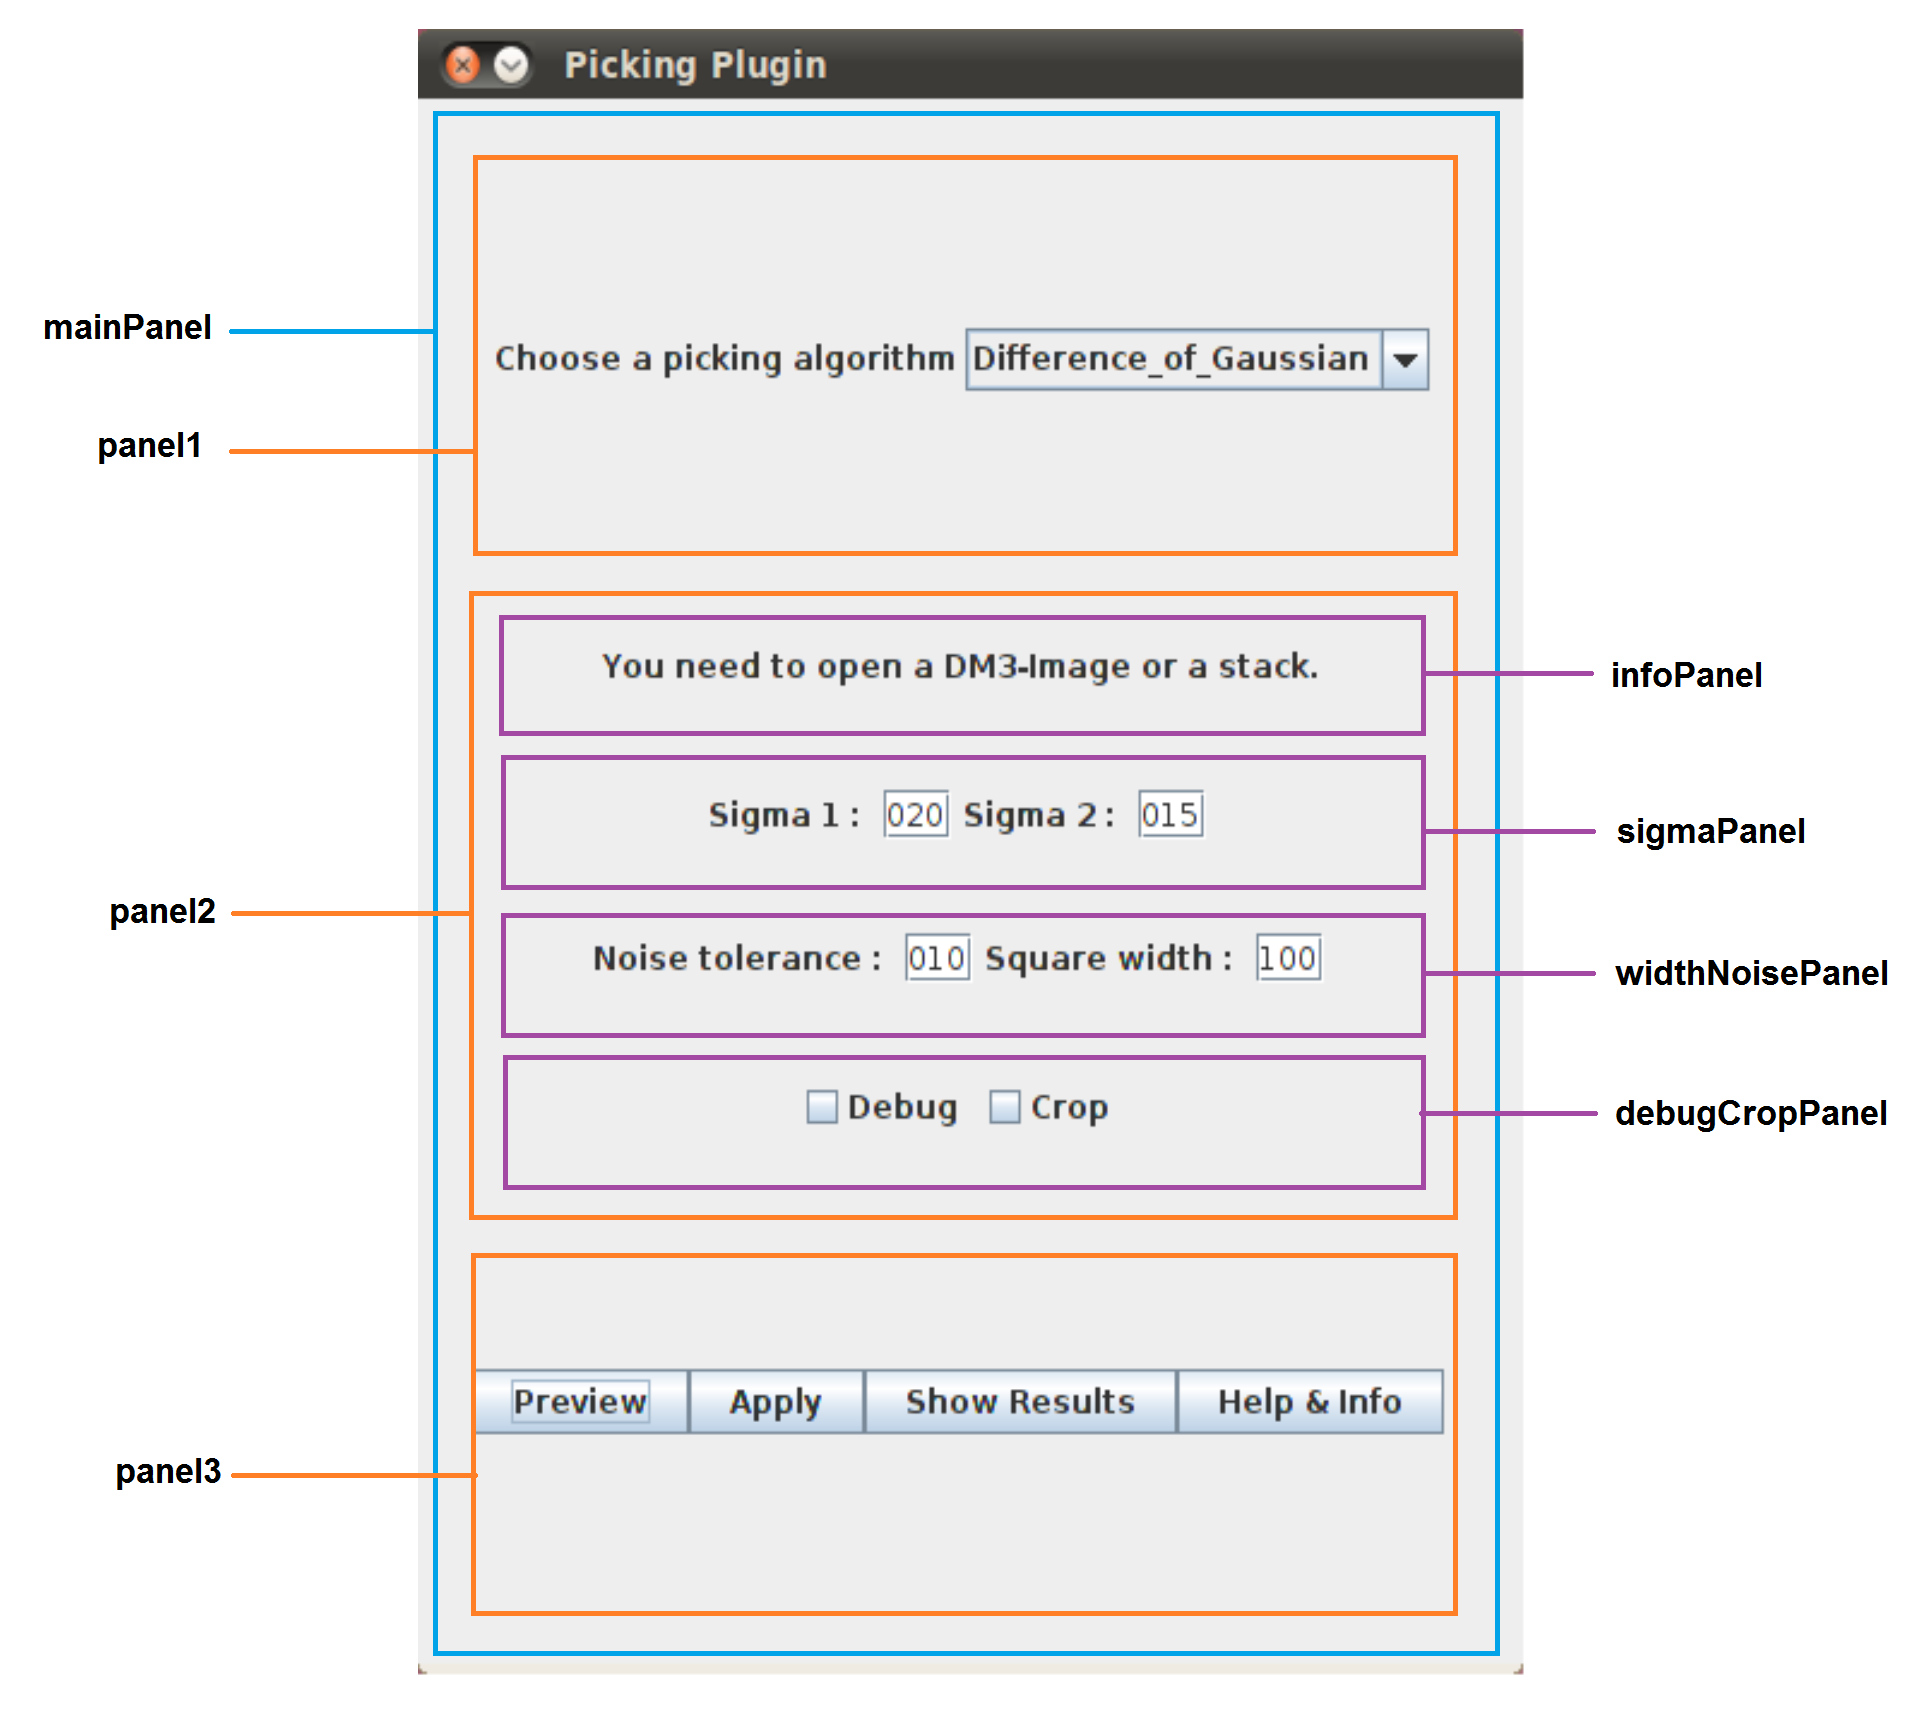
\includegraphics[width=0.8\textwidth]{plugin3-1.png}
\caption{Organisation des panels pour l'algorithme Difference of Gaussian}
\label{panneauxDetail}
\end{center}
\end{figure}
\pagebreak

\subsection{Affichage des résultats}

Lorsque l'utilisateur a coché la case "crop" avant de lancer la procédure de piquage, la classe \texttt{PickFrame} fait appel à la classe \texttt{Cropper} permettant de créer un stack. Les paramètres d'entrée de \texttt{Cropper} sont une \emph{ImagePlus} (image courante du stack) et un tableau de doubles contenant les coordonnées des particules sélectionnées. \\
A partir de ce tableau, la méthode \texttt{crop()} de \texttt{Cropper} fait appel à la méthode \texttt{setRoi()} d'\imj ~afin de retenir une zone carrée autour de la sélection. Cette zone va ensuite être dupliquée et ajoutée au stack sous la forme d'un \emph{ImageProcessor}. \\

Par ailleurs, les résultats de la sélection peuvent être affichés sous la forme d'une \texttt{ResultsTable} si on clique sur le bouton "Show Results". Elle est construite grâce au tableau de doubles cité précédemment, qui est le paramètre d'entrée de la fonction \texttt{generate-} \texttt{CsvFile()}. 

\section{Récupération des paramètres}

Le singleton de la classe \texttt{Attributes} contient une table de hashage (\emph{HashTable}) dans laquelle sont stockés tous les paramètres entrés par l'utilisateur. Ces derniers sont accessibles grâce à des clés et donc réutilisables dans les algorithmes. Le mot-clé  \texttt{synchronized} dans la fonction \texttt{getInstance()} empêche toute instanciation multiple. 

\section{Algorithmes}

Lorsque l'utilisateur fait le choix d'un algorithme de piquage parmi ceux qui lui sont proposés, cela fait appel à la classe \texttt{AlgoFactory} contenant plusieurs méthodes switch :
\begin{itemize}
\item \texttt{getPickPanel()} permet de récupérer le nom de l'algorithme choisi et d'afficher le panel2 correspondant.
\item \texttt{getPicker()} permet de lancer le piquage lorsque l'utilisateur appuie sur le bouton Apply.
\item \texttt{getPickerPreview()} permet de lancer le piquage lorsque l'utilisateur appuie sur le bouton Preview.
\end{itemize}

Une fois le panel2 chargé, l'appel aux procédures de piquage ne peut se faire que si l'on clique sur les boutons de prévisualisation (Preview) ou d'application à l'ensemble du stack (Apply). Les paramètres entrés par l'utilisateur sont sauvegardés dans la table de hashage grâce à la fonction \texttt{getInstance()} de la classe \texttt{Attributes}, puis récupérés, pour l'algorithme, par la fonction \texttt{setAttributes()} de la classe \texttt{PanelDoG} (pour suivre notre scénario). L'algorithme est ensuite appelé par la méthode \texttt{sliceSelection()} (Apply) ou par \texttt{picking()} (Preview). \\

La méthode \texttt{picking()} donne l'image courante du stack en paramètre de la méthode \texttt{pick()} alors que \texttt{sliceSelection()} parcourt le stack et appelle \texttt{pick()} autant de fois qu'il y a d'images dans le stack. \\

La méthode \texttt{pick()} quand à elle permet de lancer l'algorithme sur la sélection. Elle prend une ImagePlus et le numéro de l'image dans le stack en paramètres. Cette fonction récupère les paramètres entrés par l'utilisateur (grâce à \texttt{hashAttributes.get()}) et renvoie un tableau de résultats (X, Y, Slice). Voici un extrait du code de l'algorithme Difference of Gaussian :


\begin{lstlisting}
Hashtable<String, String> hashAttributes = Attributes.getAttributes();
String sigma1 = hashAttributes.get("sig1");

imp.setSlice(currentslice);
ImagePlus imp1 = new Duplicator().run(imp);

String si1 = "sigma=" + sigma1;

imp1.setSlice(currentslice);
IJ.run(imp1, "Gaussian Blur...", si1);
ic = new ImageCalculator();
\end{lstlisting}








\section{Applications}

Le résultat affiché sur l'image correspond aux positions des particules sur l'image courante, ou la dernière image dans le cas d'un stack.
L'utilisateur peut choisir d'afficher un tableau contenant les coordonnées (abscisses, ordonnées et positions dans le stack) des particules sélectionnées et pourra le sauvegarder. \\
De plus, s'il le désire, un stack contenant les particules sélectionnées aux positions obtenus est créé (éliminant les particules trop près du bord de l'image) et affiché.

\begin{figure}[ht]
\begin{center}
 \begin{minipage}{.450\linewidth}
  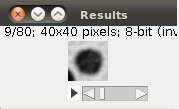
\includegraphics[width=0.75\textwidth]{cropblob.png}  
 % \caption{Difference de Gaussienne (blobs)}
 \end{minipage} \hfill
\begin{minipage}{.450\linewidth}
  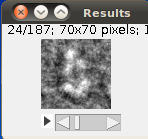
\includegraphics[width=0.5\textwidth]{cropprotDog.png}   
  %\caption{Difference de Gaussienne (protéines)}
 \end{minipage} \hfill
\caption{Exemple d'image formant le stack de particules (blobs et protéines)}
\end{center}
\end{figure}

\subsubsection*{Statistiques}

La Différence de Gaussienne permet d'obtenir les résultats suivants :

\begin{figure}[ht]
\begin{center}
 \begin{minipage}{.450\linewidth}
  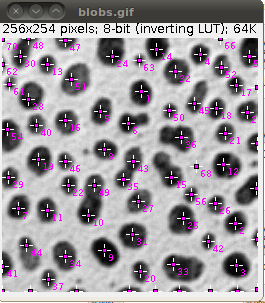
\includegraphics[width=0.75\textwidth]{blobsDog.png}  
 % \caption{Difference de Gaussienne (blobs)}
 \end{minipage} \hfill
\begin{minipage}{.450\linewidth}
  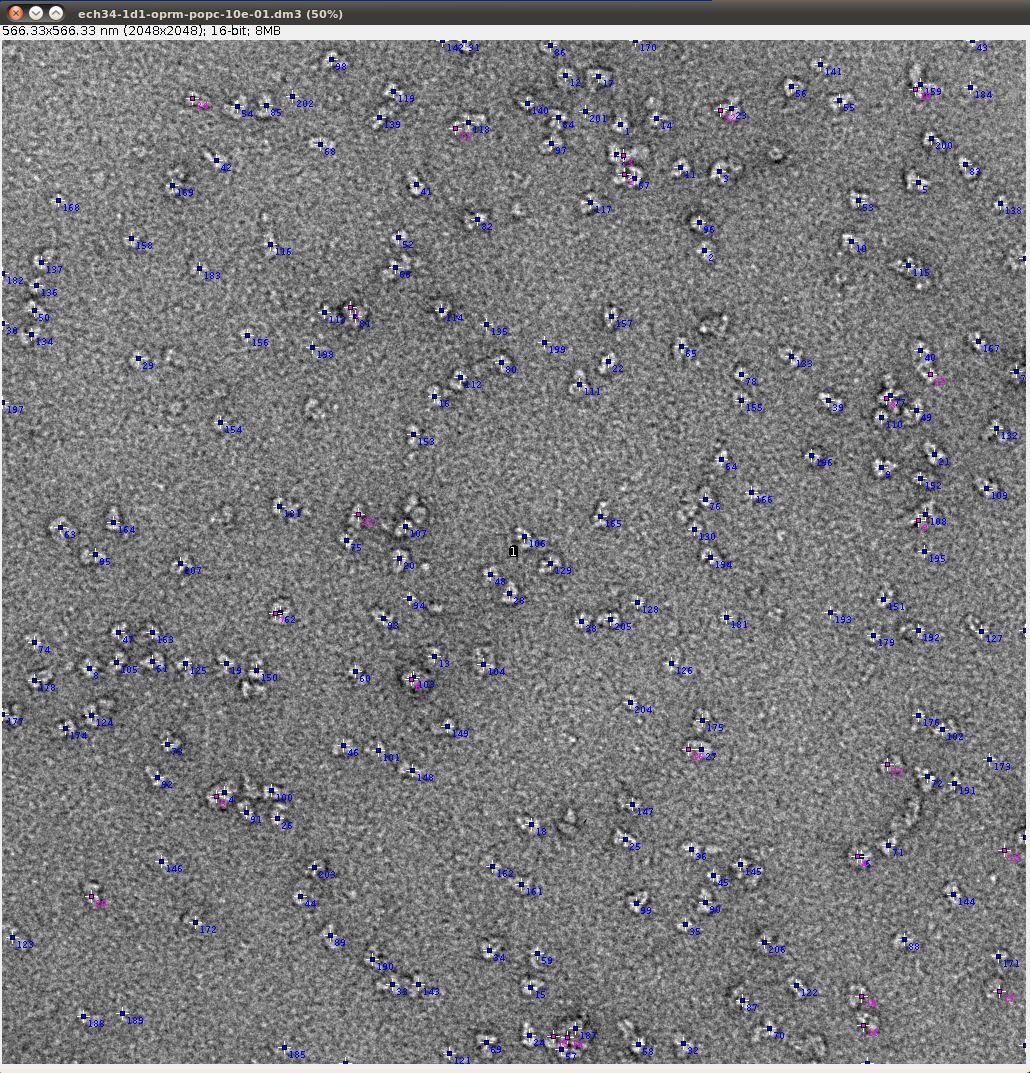
\includegraphics[width=1\textwidth]{protDog.png}   
  %\caption{Difference de Gaussienne (protéines)}
 \end{minipage} \hfill
\caption{Différence Gaussienne (blobs et protéines)}
\end{center}
\end{figure}

La Différence de dilatation permet d'obtenir les résultats suivants :


%algoFactory
%La présence d'un constructeur privé supprime le constructeur public par défaut.
%De plus, seul le singleton peut s'instancier lui même.

%attributes et algoFact
%
%Il est TRES important.



































\end{document}